\documentclass[12pt,letterpaper,twoside]{report}
\usepackage[margin=0.75in]{geometry} % set margins to 0.75 in
\usepackage{multicol}
\usepackage{multirow}
\usepackage{blindtext}
\usepackage{fancyhdr}
\usepackage{lastpage}
\usepackage{array}
\usepackage{tikz}
\usepackage{overpic}

\newcommand{\term}[2]{\noindent\hangindent=0.7cm\textbf{#1}: {#2}\par}
\newcommand{\TitleHead}{LoRa Beacon}
\newcommand{\RevisionHead}{0.0}
\newcommand{\DateHead}{23FEB2023}

\newcolumntype{R}[1]{>{\raggedleft\let\newline\\\arraybackslash\hspace{0pt}}p{#1}}

\fancypagestyle{plain}{%
  \fancyhf{}%
  \renewcommand{\headrulewidth}{0pt}% Line at the header invisible
  \fancyhead[c]{
  	\begin{tabular}{|p{3.5in}|R{3.5in}|}
	\hline
	\multirow{2}{*}{\TitleHead} &Revision\RevisionHead \\
                       & \DateHead    \\ \hline
	\end{tabular}
  }
  \fancyfoot[c]{}
  \fancyfoot[r]{ Page: \thepage \hspace{2pt} of \hspace{2pt}  \pageref{LastPage}}
}

\pagestyle{plain}



\begin{document}

%\maketitle

  	\begin{tabular}{p{2in}p{5.5in}}

	{ }&{\vspace{4in}
	
	 \Huge{LoRa Beacon}
	
	\vspace{.75in}
	
	\Large{Technical Reference}
	
	Revision\RevisionHead
	
	\DateHead
	
	
	}\\

	\end{tabular}
	


	\begin{tikzpicture}[overlay]
	\draw [draw=black, fill=black] (-.5in,6in) rectangle (.5in,-3in);
	\draw [draw=black, fill=black] (.75in,6in) rectangle (1.75in,-3in);
\node[inner sep=0pt] (Logo) at (.625in,2.5in)
    {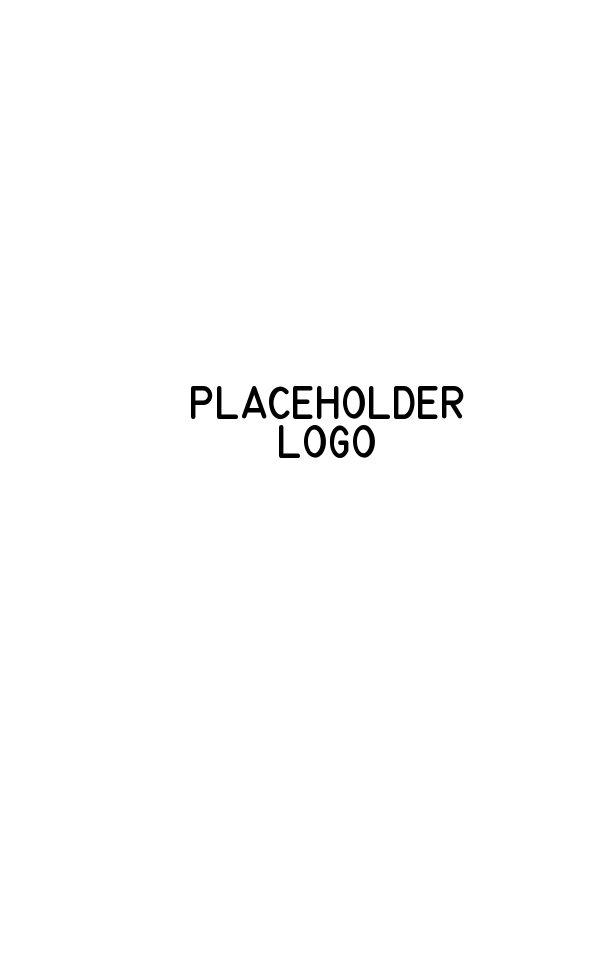
\includegraphics[width=.25\textwidth]{LoRaBeaconLogo}};

\end{tikzpicture}

\clearpage

\begin{center}
	\textbf{Bottom Line Up Front}
\end{center}
	

\tableofcontents



\chapter{Use Case}

\chapter{Theory of Operation}

\section{Modes of Operation}

\subsection{Hub Mode}

\subsection{Distributed Mode}
LoRa Beacon is an implementation of a GPS reporting system over LoRa. It targets the RNode hardware and is designed to be compatible with NIMS/ICS.

\chapter{Implementation}

\section{Phone Application}

\section{RNode Interface}

\section{Server Interface}

\section{Tracking Server}

\chapter{Future Improvements}

\chapter{Example Implementation}

\chapter{Example Control Codes}

% DEFINE DOCUMENT CONTENT HERE


\begin{multicols}{2}
[
\chapter{Terms and Acronyms}
{ }
]
\term{AGPS}{--}
\term{GLONAS}{--}
\term{GPS}{--}
\term{ICS}{See: \textit{NIMS/ICS}}
\term{LoRa}{--}
\term{NIMS}{--}
\term{NIMS/ICS}{--}


\end{multicols}



\end{document}